% Created 2016-04-14 Thu 11:02
\documentclass[11pt]{article}
\usepackage[utf8]{inputenc}
\usepackage[T1]{fontenc}
\usepackage{fixltx2e}
\usepackage{graphicx}
\usepackage{longtable}
\usepackage{float}
\usepackage{wrapfig}
\usepackage{soul}
\usepackage{textcomp}
\usepackage{marvosym}
\usepackage{wasysym}
\usepackage{latexsym}
\usepackage{amssymb}
\usepackage{hyperref}
\tolerance=1000
\usepackage{grffile}
\usepackage[inline]{enumitem} 
\usepackage{xcolor}
\hypersetup{
colorlinks,
linkcolor={red!50!black},
citecolor={blue!50!black},
urlcolor={blue!80!black}
}
\usepackage{setspace}%% The linestretch
\singlespacing
\usepackage[format=hang,indention=0cm,singlelinecheck=true,justification=raggedright,labelfont={normalsize,bf},textfont={normalsize}]{caption} % 
\usepackage{vmargin}
\setpapersize{A4}
\setmarginsrb{2.5cm}{1cm}% links, oben
{2.5cm}{2cm}% rechts, unten
{12pt}{30pt}% Kopf: Höhe, Abstand
{12pt}{30pt}% Fuß: Höhe, AB     
\usepackage{upquote}
%  use straight quotes when printing a command in minted
\AtBeginDocument{%
\def\PYZsq{\textquotesingle}%
}     
\definecolor{mintedbackground}{rgb}{0.95,0.95,0.95}   
\setlength{\parindent}{0pt}
\setlength{\parskip}{\baselineskip}
\definecolor{mintedbackground}{rgb}{0.95,0.95,0.95}
\providecommand{\alert}[1]{\textbf{#1}}

\title{\textbf{Unix Tools for Bioinformatics} (2015-06-02)}
\author{Alexander Jueterbock, Martin Jakt\thanks{University of Nordland, Norway}}
\date{*PhD course: High throughput sequencing of non-model organisms*}
\hypersetup{
  pdfkeywords={},
  pdfsubject={},
  pdfcreator={Emacs Org-mode version 7.9.3f}}

\begin{document}

\maketitle

\setcounter{tocdepth}{3}
\tableofcontents
\vspace*{1cm}









                                                



                                        

                                

















Next Generation Sequencing (NGS) data sets are big and although the data is
often text based you
simply can't open and work with them in a word processor or Excel
table - even the attempt to open a big fasta file in a text editor can
freeze your computer. Rather more importantly, even if you could, you
shouldn't as word processors are not the same as text editors. Word
processors are concerned more with the formatting of text and will store a
great deal of additional information in addition to the text that you
see. This additional information is irrelevant to the data and will in the
best case scenario make further analysis impossible. Similarly try to avoid
spreadsheets of various kinds as these almost always will try to interpret
and convert your data to something like dates or currencies or something similar.

At first, you might feel uncomfortable with the
command line but it is a very efficient and powerful tool. Moreover,
many programs to analyze NGS data can only be used from the command line and to
run them, you need to know the basic syntax. This tutorial gets you
familiar with some of the most basic command line tools and shows
you how they allow you to transfer files and how to extract
information from big files fast and easily. All tools and programs are
open source - so you will have free access to them also at your home
institution or on your private computer.


\section{Remote connection}
\label{sec-1}

To connect remotely to one of our computers, you will get:

\begin{itemize}
\item A password (e.g. PWD213)
\item A username (e.g. user)
\item An IP address (e.g. 127.0.0.1)
\end{itemize}

On `Mac' and `Linux' computers, the \texttt{ssh} (\emph{Secure Shell}) tool is
generally installed by default. To connect to a remote server, thus,
just open the command line/terminal and type:


\begin{verbatim}
ssh user@host
\end{verbatim}


Replace `user' and the IP address `host' with your own
username and the IP address of one of our remote computers.
\begin{itemize}
\item Computer 1: 158.39.60.180
\item Computer 2: 158.39.31.63
\end{itemize}

If this is the first time you want to access the remote server, you
will likely get the following warning


\begin{verbatim}
The authenticity of host '127.0.0.1 (127.0.0.1)' can't be established.
ECDSA key fingerprint is 38:59:f7:22:e5:85:ec:c3:9c:90:7x:c3:e4:ae:88:18.
Are you sure you want to continue connecting (yes/no)?
\end{verbatim}

Just type `yes' and hit enter\footnote{This is an oversimplificantion. In general you should not simply
ignore warnings like this, but it's too much off topic for us to
explain here. Note though, that you shouldn't see this warning more than once,
and if you do, you might want to read up on `man-in-the-middle attacks'.
 }. You will be asked to enter your
password. You will not see the password when you enter it, so just
type it blindly and hit enter.


\begin{verbatim}
user@127.0.0.1's password:
\end{verbatim}

When you connected successfully, you will see a \emph{welcome-text} similar to:


\begin{verbatim}
Welcome to Ubuntu 14.04.1 LTS (GNU/Linux 3.13.0-35-generic x86_64)
\end{verbatim}


If you don't only want to use the command line on the remote host, but
also want to use the Graphical User Interface to open figures,
GUI-based programs or web browsers, you should add the -X option to
your command, like:


\begin{verbatim}
ssh -X user@host
\end{verbatim}

If you use PUTTY on Windows you need to install Xming
(\href{http://www.straightrunning.com/XmingNotes/}{http://www.straightrunning.com/XmingNotes/}) and follow the guidelines
on \href{http://www.geo.mtu.edu/geoschem/docs/putty_install.html}{http://www.geo.mtu.edu/geoschem/docs/putty\_install.html}).

To open applications with a graphical user interface remotely on a
MAC, you need to install \href{http://xquartz.macosforge.org/landing/}{XQuartz}.

There are also a range of other options that let you access Unix/Linux
servers from Macs or Windows that will let you use the command line. However,
these often require specific software to be installed on the server and you
can't rely on this being the case. In general, life is just easier if you run
Linux on your own computer; is acceptable if you run MacOS and just painful
if you're stuck on Windows\footnote{This is part opinion and part fact. There are ways to use Windows to
communicate with Unix machines that are not painful and in many ways the
situation is improving. But the statement is nevertheless pretty much true
and if you are going to spend some time doing informatics you might as well
get rid of Windows as soon as you can.
 }.
\section{Basic orientation in the command line}
\label{sec-2}


The command line appears as a window/terminal similar to
Fig. \hyperref[fig-terminal]{fig:terminal}:

\begin{figure}[htb]
\centering
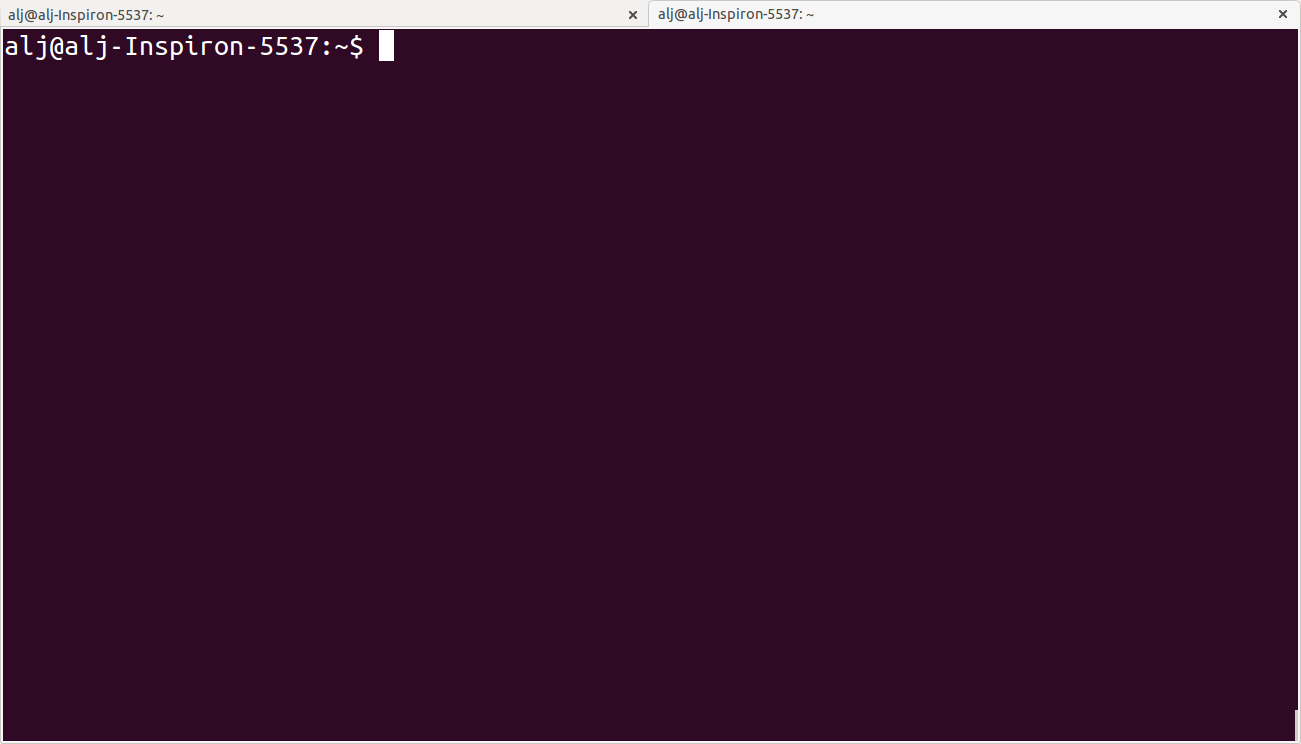
\includegraphics[width=14cm]{Terminal.png}
\caption{Command line window}
\end{figure}

The first line starts with your user name, followed by an \texttt{@} and then
the name of the computer you are working on\footnote{The beginning of the command line is referred to as the `prompt' and
like many things, it can be changed by
changing an environment variable (in this case the variable known as PS1).
 }. The line ends with a
\texttt{\$} - after this sign you can enter your commands.

The Unix cheat sheet (see at the end of this file) provides an
overview of the core commands to navigate and operate in the Unix
command line. Most commands allow you to adjust their behaviour with a
variety of so-called arguments or flags. Most of the commands, for
example, display help information if you use them with the \texttt{-{}-help}
flag.

For example, if you type \texttt{ls -{}-help}, you'll get an overview of the
common usage of the command \texttt{ls} and of the flags that can change the
behaviour of this command.  The \texttt{-{}-help} option doesn't provide much
help for the \texttt{ssh} command. In such cases you can try the \texttt{man}
command. It opens a manual page of the specified tool. For example,
try \texttt{man ssh}. If you want to leave the manual page, just hit \texttt{q}.
Before we will work on some sequencing data, let's have a look
at the commands that allow you to change directories and how to get an
overview of files that were saved in these directories.
\subsection{Directory navigation}
\label{sec-2-1}

Navigating through your directories is a big hurdle if you are new to
the command line and are used to `clicking' you way in and out of folders. To
understand how to move in and out of folders (directories on Unix/Linux) and to look at the
content of folders is an essential step to analyse your data on
the command line.
\subsubsection{Conventional directory layout}
\label{sec-2-1-1}



\begin{quote}
On a UNIX system, everything is a file; if something is not a file, it is a process.
\end{quote}

This is a simplification but it is mostly true. A directory on a Unix
system is just a file that contains names of other files. Also
programs, images and documents are all files. These files are
hierarchically ordered in a conventional tree-like structure (see
Fig. \hyperref[fig-linuxfiletree]{fig:linuxfiletree})


\begin{figure}[htb]
\centering
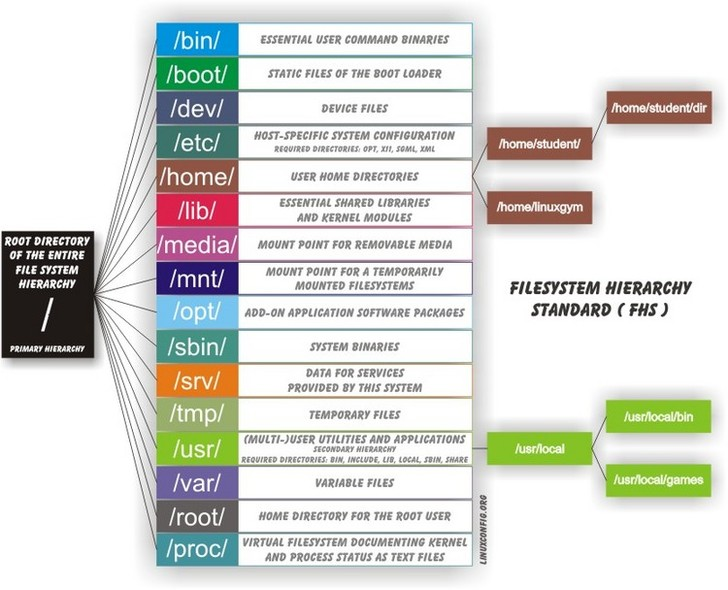
\includegraphics[width= 12cm ]{linuxfiletree.jpg}
\caption{Conventional file tree structure on a UNIX system from \href{http://linuxconfig.org/filesystem-basics}{linuxconfig.org}}
\end{figure}


The root (represented as \texttt{/}) is the top-most level of this hierarchy.
When you connect to a Unix computer, you are automatically located in
your user home directory (\texttt{/home/username/}) and this is the only one
you have write access rights to in this course. Many of the programs and
scripts that you will use in ths tutorial are located in the \texttt{/usr/}
directory, generally in \texttt{/usr/local/bin/}. 

Applications that are located in \texttt{/usr/local/bin/} can be run by any
user because this directory is automatically specified in the so-called
\texttt{PATH} variable of every user. The \texttt{PATH} vairable is simply a
variable that specifies the directories where executable programs are
located. You will meet this \texttt{PATH} variable when you learn more about
running programs.
\subsubsection{Moving in and out of directories with \texttt{cd}}
\label{sec-2-1-2}

 \texttt{cd} stands for `change directory'. with this command you can navigate
 in and out of your directories. To see what your present working
 directory is, simply type \texttt{pwd} (for `present working directory') and
 hit enter


\begin{verbatim}
pwd
\end{verbatim}

 The response in my case is:


\begin{verbatim}
/home/alj/
\end{verbatim}

 When you want to `move' to a different directory, the TAB key comes in
 handy as it auto-completes the possible sub-directories you can `move'
 to. For example, when you type \texttt{cd} and hit the TAB key twice, you get an
 overview of all possible sub-directories. For example,


\begin{verbatim}
cd 
.adobe/
Adobe/
.cabal/
.cache/
.compiz/
.config/
--More--
\end{verbatim}

 Hit ENTER to see more sub-directories in your shell or `n' to leave the
 list of sub-directories.

 If you know that your target sub-directory starts with the letters
 `Do', you can type these after the \texttt{cd} command and then hit TAB twice
 (once is enough if there is only one sub-directory that starts with the
 letters `Do'):


\begin{verbatim}
cd Do
Documents/ Downloads/
\end{verbatim}

 I, for example, have two directories starting with `Do', \texttt{Documents}
 and \texttt{Downloads}. So, TAB completion helps when moving into
 sub-directories, but how to get out of them again? With


\begin{verbatim}
cd ..
\end{verbatim}

 you move one level up in your hierarchical directory structure.  If
 you want to go to your home directory from wherever you are, use


\begin{verbatim}
cd ~
\end{verbatim}

 or just
 

\begin{verbatim}
cd
\end{verbatim}
\subsubsection{Tip}
\label{sec-2-1-3}

If there are empty spaces in your filepath, you need to precede them
with a backslash (=\=) in order to navigate to them, like in 


\begin{verbatim}
/home/my\ directory/
\end{verbatim}

or use quotation marks


\begin{verbatim}
cd "/home/my directory"
\end{verbatim}
\subsubsection{What is saved in the current directory?}
\label{sec-2-1-4}

 Once you navigated with \texttt{cd} to your target directory and you want to
 look at the files and sub-directories that are located in it, you can
 use the command \texttt{ls} and hit enter. The tool \texttt{ls} comes with many
 options that refine the way that the results are shown; you get an
 overview of these options with:


\begin{verbatim}
ls --help
\end{verbatim}

 The combination of options that I use most frequently are


\begin{verbatim}
ls -lhcrta
\end{verbatim}

 The option
\begin{itemize}
\item \texttt{-l} provides additional information to the file or folder name
\begin{itemize}
\item file permissions
\item user and group owners of the file
\item size
\item date of modification
\end{itemize}
\item \texttt{-h} prints the file sizes in human readable format, like 100K instead of 102400
\item \texttt{-c} sort by last modification of file status information
\item \texttt{-r} reverse order while sorting (so that the newest files are the last that are printed)
\item \texttt{-t} sort by modification time, newest first
\item \texttt{-a} prints also the hidden files (starting with a dot `.').
\end{itemize}
  
\subsubsection{Have a look at the directory structure}
\label{sec-2-1-5}

The command line tool \texttt{tree} prints the hierarchical structure of your
files and directories (recursing into all sub-directories) to the screen.

 To discriminate files from folders via colors, use the \texttt{-C} option


\begin{verbatim}
tree -C
\end{verbatim}

 To show only directories, use the \texttt{-d} option


\begin{verbatim}
tree -d
\end{verbatim}

 

Try also the following command:


\begin{verbatim}
tree -sh
\end{verbatim}

Here, 
\begin{itemize}
\item \texttt{-s} provides the file and directory sizes
\item \texttt{-h} prints the sizes in a human readable format
\end{itemize}
\subsubsection{Tip}
\label{sec-2-1-6}

Besides the TAB-key, that allows for auto-completion of commands or
filenames, the UP- and DOWN-arrow keys on your keyboard can safe you
some time. These buttons allow you to navigate through the history of
command that you have entered in the command line.  Try it out.
\subsubsection{Create, move and remove files and directories}
\label{sec-2-1-7}

New directories can be created with


\begin{verbatim}
mkdir directoryname
\end{verbatim}
Here, \texttt{directory} is the name of the directory you want to create.

To create a new empty file, use the command \texttt{touch}:


\begin{verbatim}
touch filename
\end{verbatim}

You can move or rename files with the command \texttt{mv}. For example:


\begin{verbatim}
mv file1 file2
mv file1 ../file1
\end{verbatim}

The first command renames file1 to file2. The second command moves
file1 one folder up.

If you don't want to move but copy a file, use the command \texttt{cp}.


\begin{verbatim}
cp file1 file2
\end{verbatim}
Instead of renaming file1 to file2, as the \texttt{mv} command does, the \texttt{cp}
command keeps file1 and creates a new file2 with the same content.

The most dangerous command that you learn to day is \texttt{rm}, which stands
for remove. If you remove a file with this command, it is gone and you
can not retrieve it. But if this is what you want, you can remove, for
example, file2 that we created above with the following command:



\begin{verbatim}
rm file2
\end{verbatim}

To remove an entire directory, use \texttt{rm} with the \texttt{-r} flag, like:


\begin{verbatim}
rm -r directoryname
\end{verbatim}
\subsubsection{Tip}
\label{sec-2-1-8}

To get an overview of all the commands that you have used before, just
type



\begin{verbatim}
history
\end{verbatim}

and hit ENTER.
\subsection{Data transfer between computers}
\label{sec-2-2}

Before you can work on a remote server with your own data, you first
need to know how to transfer them.  One of the best
platform-independent GUI programs that allows you to up- and download
files is FileZilla (Download and Documentation:
\href{https://filezilla-project.org/}{https://filezilla-project.org/}). In the following lines I want to
introduce the command line tools \texttt{rsync} and \texttt{sftp/lftp}, that allow
you to transfer and synchronize files.
\subsubsection{rsync}
\label{sec-2-2-1}



 \texttt{rsync} stands for ``remote sync''. This powerful tool has plenty of
 options.  Here is the most basic syntax to transfer files from a
 \emph{source} (SRC) location to a \emph{destination} (DEST) with \texttt{rsync}. (Text
 in square brackets denotes optional arguments, in this case optional
 options!)


\begin{verbatim}
rsync [OPTIONS] SRC DEST
\end{verbatim}

 SRC and DEST can either be files or folders. For example, to
 transfer the file `file.txt' from your local home folder to a remote
 server, you can type:


\begin{verbatim}
rsync --progress /home/user/directory/file.txt user@host://home/user/
\end{verbatim}

 Here, you need to change \texttt{/home/user/directory/} to your own filepath and
 \texttt{file.txt} to your own filename. In `=user@host=', \texttt{user}
 represents your username on the remote server and \texttt{host} the IP
 address of the remote server.  The \texttt{-{}-progress} option will indicate
 the progress of the file transfer - which is useful when transferring
 big files.

 If you want to transfer files from the remote server to your
 local computer, just swap the source and destination path
 specifications:


\begin{verbatim}
rsync --progress  user@host://home/user/file.txt /home/user/directory/
\end{verbatim}

 If you want to transfer all files that are located in your local
 folder \texttt{/home/user/directory/}, you can use the following command


\begin{verbatim}
rsync -avz --progress /home/user/directory/ user@host://home/user/
\end{verbatim}

 Here,
\begin{itemize}
\item \texttt{-av} will transfer the files in `archive mode' (which combines
   several options, including recursing into directories)
\item \texttt{-z} will compress the files durig the transfer
\end{itemize}

 Note the trailing slash after the source directory:
 \texttt{/home/user/directory/}. If you do not use this trailing slash, like
 \texttt{/home/user/directory}, then \texttt{rsync} will create a folder with the
 name \texttt{directory} at the destination and copy all files from the source
 folder into it.


Ok, that's all we need to know to get the sequencing data from last
week to the remote computer. As we need the data in the following
tutorials, it is best if you upload them now.
 
\subsubsection{sftp/lftp}
\label{sec-2-2-2}

rsync is a wonderful tool, but its power makes it complex and it can be
difficult to remember how to do even simple things (try \texttt{man rsync} if
you don't believe me!). When using rsync you also need to know and
remember where the files and directories that you wish to synchronise
are located. My preference is for using
the programs similar to the old ftp command line client (which even Windows has). 
This provides an
environment very similar to the normal Unix shell, where you change
directory using \texttt{cd}, list the files using \texttt{ls}, find out where you are
using \texttt{pwd} and so on. However, the ftp protocol is inherently insecure;
it may not matter that the data is transmitted without encryption, but
you should be concerned about sending your password in plain text
across the ethernet. Not good. Hence, these days we use the sftp (secure
file transfer protocol) instead. On Mac and Unix systems you will
essentially always have the sftp command line client installed. On
Windows, well, you can use Putty or other third party tools. On Linux
systems you may also have the lftp command line client installed. Its
usage is almost identical to the usual sftp and ftp clients but it comes
with extended functionality that allows you for example to mirror (i.e.
synchronise directories) between the remote and local computers.

To use the sftp program, simply type:


\begin{verbatim}
sftp hostname
\end{verbatim}

into your terminal. The hostname may need to be specified as the IP
address (a load of numbers) or can be a simple name depending on your
setup. After the connection is made you will be asked for your password.
The sftp program assumes that you will be using the same username as you
are using on the local computer. If this is not the case you can specify
your username by:


\begin{verbatim}
sftp username@hostname
\end{verbatim}

After having successfully logged in to the remote computer you can move
around the directories as if you were logged in over a shell session
(i.e. using \texttt{ls}, \texttt{cd} and so on). If you wish to change the directory
on the local machine, simply use the \texttt{lcd} command. You can also run
commands in your local shell by prefixing these with an !, eg. \texttt{!ls} or
\texttt{!pwd}. You can create directories on the remote computer with \texttt{mkdir},
and on the local machine with \texttt{!mkdir}. To transfer files from the
remote to the local computer use \texttt{get fname}. You can use globbing (*)
to expand the file set, eg. \texttt{get *.fa} for all files ending in `.fa'.
(For this you may need to use \texttt{mget *.fa} on some implementations, this
used to be true on the old ftp command line client). Similarly you can
upload files using \texttt{put}.

As mentioned lftp is almost identical in its operation. However, when
starting the program you need to specify that you wish to use the sftp
protocol as it defaults to the standard ftp protocol (with an anonymous
user). Hence use something like:


\begin{verbatim}
lftp sftp://username@hostname
\end{verbatim}

lftp also allows you to mirror whole directory structures using the
\texttt{mirror} command which can save you a lot of time. Finally, when I
started using lftp, the standard ftp and sftp clients did not provide
tab completion, and this was a big advantage of lftp at that time. These
days most if not all of the clients provide this functionality, so it is
not quite as big a deal as it was in the long past.
\subsubsection{Tip}
\label{sec-2-2-3}


If you want to transfer in one go, all files that have some common
characteristic in their name you can use the asterisk \texttt{*}, which
stands for `any character'. The \texttt{*} is one of the most commonly used
wildcard symbols that stands for a continuous string of characters. To
specify a set of filenames with wildcard characters is also referred
to as \emph{globbing}.

For example, if you want to transfer all
fasta files at once, you can use


\begin{verbatim}
rsync -avz --progress /home/user/directory/*fasta user@host://home/user/
\end{verbatim}
This means that any characters can precede the \texttt{fasta} file ending



If you want to transfer all files that belong to a certain population
and are, for example, marked with `Pop1' in the file name, you can use:


\begin{verbatim}
rsync -avz --progress /home/user/directory/*Pop1* user@host://home/user/
\end{verbatim}
This means that any characters can precede or follow the \texttt{Pop1}
character in the file name.
\section{Running programs (and the PATH variable)}
\label{sec-3}


When using the shell you normally run a program by simply typing the
program name and any required arguments. But how does the shell know
what program to run and where to find it? On a typical Unix / Linux
system executable files (i.e. programs) can be found in a range of
standard locations (eg. \texttt{/bin/, /sbin/, /usr/bin/, \textasciitilde{}/bin/}) as well as
anywhere a user puts them. Normally when you run a program by simply
typing its name, the shell will look for an executable file of that name
in a list of directories specified by the \texttt{\$PATH} environment variable.
The first matching program is then run.

The user can also directly specify the location (path) of the
executable; this is necessary if the program you wish to run is not
present in any directory specified by the \texttt{\$PATH} variable, or if
multiple programs of the same name are present and you want to run one
of the later matches:


\begin{verbatim}
/usr/local/bin/pg_ctl start
\end{verbatim}

to start a version of the Postgresql database installed in
/usr/local/bin specifically.

You can also specify a path that is relative to your current location.
If for example your current working directory is
\texttt{\textasciitilde{}/Documents/testPrograms/} and you wish to run a locally installed
version of gcc (gnu C compiler) found in \texttt{\textasciitilde{}/bin/}:


\begin{verbatim}
../../bin/gcc -o test main.c
\end{verbatim}

(Remembering that ../ takes you up one level in the directory
structure). To do the same you could also make sure that the \texttt{\$PATH}
contains \~{}/bin before other potential locations of gcc.

To check the current value of your \texttt{\$PATH}, simply use the echo command:


\begin{verbatim}
echo $PATH
\end{verbatim}


To learn how to extend your own PATH variable have a look in the hidden
.basrc or .bash$_{\mathrm{profile}}$ file in your home directory. It usually gives a
few examples. Failing that have a look at Google.

Finally if you've written a small script or installed a program in your
current working directory you can run that by typing \texttt{./scriptname}. There
is nothing special about that, it is merely how you represent the
relative path to your current working directory.
\section{Retrieving basic information from common NGS files}
\label{sec-4}

 
Now that we know how the commandline works, how we can change
directories and transfer files, it's time to look at NGS data output
and to learn how to open and summarize information from such files -
like, for example, the number of sequences in a fasta file.

The folder PracticeFiles contains the following files:
\begin{itemize}
\item HTS.fasta and HTS2.fasta, fasta files with sequence identifiers and sequences
\item HTS.fastq, a file with sequences and associated base qualities
\item HTS.sam, an alignment file
\end{itemize}
\subsection{Uncover the content of a file and search for patterns}
\label{sec-4-1}

The tool \texttt{less} can be used to display the content of text files one
line or page after the other. Since it doesn't read the entire content
of a file at once, it is very useful for looking into large files.

Let's have a look at a fastq file with the command:


\begin{verbatim}
less Fastqfile.fastq
\end{verbatim}

Once you have opened a fasta file, for example, with \texttt{less} \ldots{}


\begin{verbatim}
less Fastqfile.fasta
\end{verbatim}

\ldots{} you can search for patterns, like the nucleotide sequence `GCTC', with \texttt{/}, like


\begin{verbatim}
/GCTC
\end{verbatim}

hitting \texttt{n} repeats this search on the remainder of the file.

To show only those lines in the file that match the nucleotide
sequence `GCTC', type this sequence after the \texttt{\&} sign:


\begin{verbatim}
&GCTC
\end{verbatim}
 
To go to the last line of the file, just type \texttt{G}, to go to the first
line, type \texttt{g}. To close the file again, hit \texttt{q}.


The \texttt{less} command has more options than this. You get an overview of
these with the \texttt{-{}-help} flag:


\begin{verbatim}
less --help
\end{verbatim}


The \texttt{head} command, followed by the name of a text file, prints by
default the first 10 lines/rows of the file to the terminal.  The \texttt{-n}
option allows to determine the number of rows that shall be
printed. For example, to extract the first sequence-id along with the
nucleotide sequence from HTS.fasta, you can select the first two lines
with:


\begin{verbatim}
head -n 2 HTS.fasta
\end{verbatim}

When the line number \texttt{K} is preceded with \texttt{-}, then all but the last \texttt{K}
lines are printed. For example, the command to print all but the last
ten lines from a HTS.fasta is:


\begin{verbatim}
head -n -10 HTS.fasta
\end{verbatim}

The \texttt{tail} command, in contrast, prints by default the last 10 lines
of a file to the terminal. Also here you can select the number of
lines with the \texttt{-n} option. When the line number \texttt{K} is preceded by a
\texttt{+}, then all but the first \texttt{K} lines are printed.  For example, to
exclude the first two lines from HTS.fasta


\begin{verbatim}
tail -n +2 HTS.fasta
\end{verbatim}


To extract specific lines from a file, the tool \texttt{sed} can help you. To
print all lines between line 234 and 236 from HTS.fasta, for example, use:


\begin{verbatim}
sed -n '234,236p'
\end{verbatim}
\subsection{Counting words, lines, and characters with `wc' and searching for patterns with `grep'}
\label{sec-4-2}

If you want to get a rapid overview of the number of lines in a file,
the \texttt{wc} command is the right tool. In output-files where
every line represents a sequence, for example, \texttt{wc -l} is all you need to count the
number of sequences.


\begin{verbatim}
wc -l File.txt
\end{verbatim}

The \texttt{-l} option specifies that you want to count the number of
lines. The \texttt{-m} and \texttt{-w} options further allow you to count the number
of characters or words.


To count the number of sequences in a fasta file, you have to limit
the lines that are counted to those starting with a ``>'' sign
because ``>'' precedes every sequence identifier:


\begin{verbatim}
>SEQ1_ID
GGATTCATAGAAACCATAGATACATAGATACATAGATTAGGGACAGATAATAG
>SEQ2_ID
GATTTGGGGTTCAAATTAGTATCGATCAAATAGTAAATCCATTTGTTCAACTC
>SEQ3_ID
AGATACAGAGAGACAAGACATAGACAGATAACAGAATAGAGATAGAGGAGAGG
\end{verbatim}

\texttt{grep} allows you to extract lines that contain specific
characters, like ``>''. 


If you type


\begin{verbatim}
grep ">" HTS.fasta
\end{verbatim}

All lines in HTS.fasta that contain the ``>'' character are printed to
the screen. You can stop the flow of output by pressing Ctrl+C. If you
don't want to write these lines to the screen but want to count them,
the \texttt{|} symbol provides a `pipe' to pass the output from the \texttt{grep}
command to the \texttt{wc} command. So, to count the number of
sequences in HTS.fasta, you can use the following command:


\begin{verbatim}
grep ">" HTS.fasta | wc -l
\end{verbatim}

Here a recap on what the commands mean: \texttt{grep} is used to search for
\texttt{>} signs in the fasta file. All sequence-id's start with this
character. Instead of printing all these lines to the terminal, we
re-direct it to the \texttt{wc} command with the pipe symbol \texttt{|}. Using the
\texttt{-l} option, \texttt{wc} counts all the lines. Here, \texttt{wc} doesn't need an
input file.


Your turn. What command would you use to count the number of sequences
in a fastq file? 


If you are in doubt what quality encoding your fastq file has, \texttt{grep}
can help you. Have a look at Fig. \hyperref[Fig-QC]{Fig:QC}. If you find one of the ASCII
characters 33 (character'!') to 58 (character `:'), you can be sure
that the quality encoding is Phred+33. 


\begin{figure}[htb]
\centering
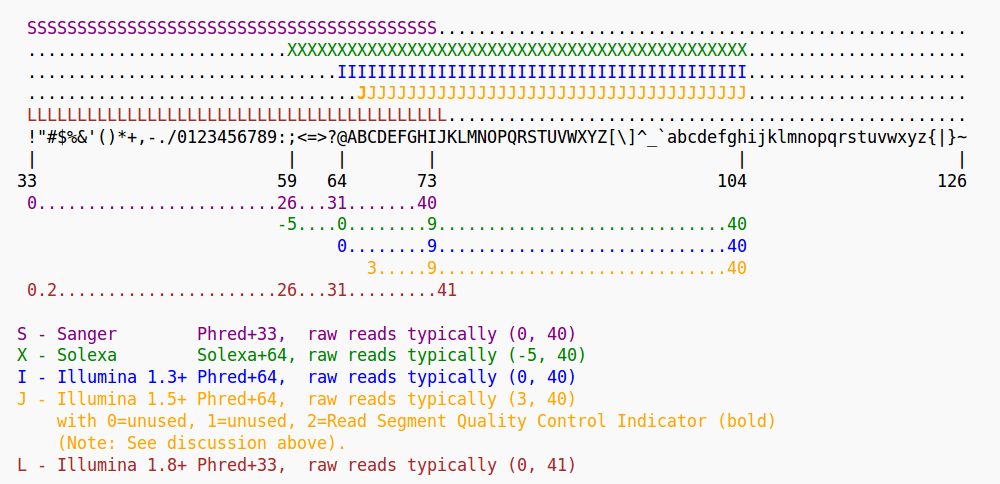
\includegraphics[width=14cm]{Fastq.png}
\caption{Quality score encodings}
\end{figure}


So, try if you find one of the Phred+33-specific quality characters in
HTS.fastq. For example:


\begin{verbatim}
grep "!" HTS.fastq | wc -l
\end{verbatim}



\texttt{grep} also allows you to search for the sequence of a specific
gene-id and identify the line of the hit in a fasta file, if you use
it with the \texttt{-n} flag. For example, if you want to know which line
in the HTS.fasta file holds the sequence with the gene-id
`gi|612475216|gb|AZHG01011862.1|', you can use:


\begin{verbatim}
grep -n "gi|612475216|gb|AZHG01011862.1|" HTS.fasta
\end{verbatim}

It is line 23724.
\subsection{INFO on regular expressions}
\label{sec-4-3}


\texttt{grep} stands for \emph{global regular expression printer} and is a
command-line utility for searching plain-text data for lines matching
a regular expression. With regular expressions you can match strings
that are not identical but follow a specified pattern.  We won't
go into further detail here, but you can read more about regular
expressions in \href{http://www.scootersoftware.com/RegEx.html}{A Tao of Regular Expressions} and you can find a 
short introduction in the Perl section below. Also, \href{http://www.cheatography.com/davechild/cheat-sheets/regular-expressions/}{here} you will find
a cheat sheet with essential regular expressions.
\subsection{Combine the content of files with `cat' and `>'}
\label{sec-4-4}

The most common use of the \texttt{cat} command is to redirect the contents of
text files to other files or commands.

The following command, for example prints the content of HTS.fasta to the screen


\begin{verbatim}
cat HTS.fasta
\end{verbatim}

With the \texttt{>} and \texttt{>>} operators, you can print the content of files
not to the screen but to other files. This allows to rapidly combine
two files, even huge ones. For example, in the following command
\texttt{HTS.fasta} and \texttt{HTS2.fasta} are combined to
\texttt{COMBINED.fasta}.


\begin{verbatim}
cat HTS.fasta > COMBINED.fasta
cat HTS2.fasta >> COMBINED.fasta
\end{verbatim}

The \texttt{>} operator redirects the output of the \texttt{cat HTS.fasta}
command (the content of \texttt{HTS.fasta}) to \texttt{COMBINED.fasta}. The
\texttt{>>} operator adds the output of the \texttt{cat HTS2.fasta} command to
the \texttt{COMBINED.fasta}. If we would use the \texttt{>} operator instead of
the \texttt{>>} operator in the second line, the content of
\texttt{COMBINED.fasta} file would be overwritten, not appended. So, the \texttt{>}
operator (over) writes content to a specified file while the \texttt{>>}
operator appends content to a specified file. If you use the \texttt{>>}
operator, the specified file needs to exist already.
\subsection{Counting filtered reads in SAM files with `awk'}
\label{sec-4-5}

Later in the course we will encounter specific programs that can filter
SAM and VCF files. Here, I want to show you that we can also use basic
command line tools to filter such files.  The command line tool \texttt{awk}
can extract single columns or apply a filter on column values in
any file that is organized in columns - as SAM and VCF files
are. The \texttt{-F} option allows you to specify if your columns are
delimited by commas, spaces, tabs or any other character.

We learned this morning that SAM files (alignment files) are
 tab-delimited (\texttt{\textbackslash{}t} and always contain the mapping quality in the
 fifth column (\texttt{\$5}). Thus, to count mappings in a SAM file that
 have qualities > 20, we first strip off the header lines
 containing the \texttt{@} character  with \texttt{grep}:


\begin{verbatim}
grep -v "^@" HTS.sam
\end{verbatim}

Here, the \texttt{-v} option inverts our search (all lines including \texttt{@} at
the beginning of the line - specified by the \texttt{\textasciicircum{}} sign - are excluded).

The above command would print all non-header lines to the
screen. Instead, we want to pipe the output of this command to \texttt{awk},
in order to extract only those reads with a mapping quality >20 and
then pipe this output to \texttt{wc} to count the lines:


\begin{verbatim}
grep -v "^@" HTS.sam | awk -F "\t" '$5 > 20 {print $0}' | wc -l
\end{verbatim}

Here, \texttt{\$0} refers to the entire row, while \texttt{\$5} refers to column 5 of
that row. \texttt{-F} just specifies the field separator, and
\texttt{\textbackslash{}t} sets it to the TAB character. Since we pipe (using \texttt{|}) the output of \texttt{grep} to
\texttt{awk}, and then the ouput of \texttt{awk} to \texttt{wc} the lines are not printed to screen but directly
counted with the \texttt{wc} command. Only the output of \texttt{wc} gets printed to the screen.
\subsubsection{Variables in Perl}
\label{sec-5-1}


In order to handle information within a program we assign values to
variables and then manipulate these according to the flow of the
program. Perl provides three different types of variables:

\begin{itemize}
\item Scalar variables: these take a single value (usually a number or some text) 
   and are denoted by a \texttt{\$} prefix, eg. \texttt{\$var}.
\item Arrays: these contain an ordered series of values that are accessed by their
   position. Arrays are denoted by an \texttt{@} prefix, eg. \texttt{@array}.
   Individual values are accessed as scalars, using square brackets to
   indicate the position, eg. \texttt{\$array[3]} accesses the fourth element of
   \texttt{@array} (the fourth rather than the third as we count from 0).
\item Hashes (or associative arrays): these hold key-value pairs and are
   denoted by the \texttt{\%} prefix, eg. \texttt{\%hash}. Individual elements are again
   accessed as scalars, but this time using curly brackets, eg.
   \texttt{\$hash\{key\}}. The key value can be anything that can be assigned to a
   scalar (numbers, text, and references).
\end{itemize}
\subsubsection{Assigning variables}
\label{sec-5-2}


The values of variables can be assigned directly in the program's source
code, but are more frequently assigned through the command line
arguments (see below) or by the program reading input (data or
configuration) files (see lower section). Scalars are the simplest:


\begin{verbatim}
$var1='hello'; 
$var2="world";
$var3=3.14;
\end{verbatim}

Strings (i.e. text elements) can be assigned using either single \texttt{’} or
double `` quotes. The use of double quotes expands variables within the
quoted text such that:


\begin{verbatim}
$var4="goodbye $var1";
\end{verbatim}

will assign the text ``goodbye world'' to the variable \texttt{\$var4}.
In contrast:


\begin{verbatim}
$var4='goodbye $var1';
\end{verbatim}

will assign the text `goodbye \$var1' to \texttt{\$var4} (without the quotation
marks!).
Double quotes also allow escape codes such as \texttt{\textbackslash{}n \textbackslash{}t} to be interpreted
as newline and tab characters respectively.

Arrays can be assigned in a number of ways, occassionally directly in
the code:


\begin{verbatim}
@ar1 = (1, 2, "three");
\end{verbatim}

An empty array can also be created and then extended by adding elements.
This can be done by either using the \texttt{push} function or by using
subscripts beyond the range of the array:


\begin{verbatim}
## text following a # character are treated as comments

@ar1 = (); ## creates an empty array of length 0 
push @ar1, "hello"; ##extends this array to have a length of 1

$ar1[2] = "three"; 
## the array now has a length of three, but an undefined value in the second position 
## $ar1[1]
\end{verbatim}

In most cases, elements of an array will be assigned to values found in
input files containing the data to be analysed, rather than being
defined directly in the code as above.

Hashes (associative arrays) that store key value pairs are defined in a
similar way to arrays. Again the actual values are usually obtained from
input files, but can also be defined in the code.


\begin{verbatim}
%kv1 = ();
## this creates an empty hash structure. It is actually not necessary to
## declare it, but one can directly assign elements of the hash:
$kv1{1} = "one";
$kv1{2} = "two";
$kv1{'three'} = 3;

## this hash could also have been created in a single line :
%kv1 = (1 => "one", 2 => "two", 'three' => 3);

## to access the elements of an associative array we obtain
## the keys of the hash using the keys command.

@keys = keys %kv1;
## print the first value associated with the first key:
print "$keys[0] $kv1{$keys[0]}\n";

## the \n simply defines a newline character
\end{verbatim}


Scalars, arrays and associative arrays can be combined to create
arbitrarily complex data structures. Hence you can have hashes of arrays
and arrays of hashes and so on. To fully use more complicated data
structures requires an understanding of the reference. A reference is a
value that points to another piece of data by providing the memory
address of that data. For example, an array of hashes is encoded as an
array of references to hashes. To obtain the value of data referred to
by a reference it the reference must be dereferenced. Perl has
a number of different ways in which this can be done, but these will not
be explained in depth here as it can get a bit messy. 

Semicolons: you may have noticed that in the above examples almost every
line ends with a semicolon. In Perl (and in many other languages), the
semicolon is used to denote the end of statements. This means
that single statements can be spread across several lines and that a
single line can contain a number of statements. This can greatly aid the
readability of the code.
\subsubsection{Data types}
\label{sec-5-3}


In the above examples we assigned values to variables without caring
about what kind of data we used. For example consider the following:


\begin{verbatim}
$var1 = "one";
$var2 = 2;
$var3 = $var1 + $var2;  ## !!??!!
\end{verbatim}

Here we have assigned the value of \texttt{\$var1} to a piece of text (which we
will refer to as a string from here on) whereas \texttt{\$var2} has been
assigned a numeric value. Perl is a dynamically typed language; that
means that you do not have to explicitly define what type of value a
variable contains. This is convenient when writing a script (essentially
a small program), but this does make it easier to make mistakes in more
complicated situations. In the above example, the third line doesn't
make sense, and will generate an error. In this case it is obvious from
the code, but in most real world situations the values will be read in
from an external file produced by some other program or person in which
case finding the reason for the problem may not be so simple.

Perl essentially has three data types, strings, numeric values and
references. References are necessary for making more complex data
structures and to allow variable values to be modified by functions. As
mentioned above though, references will not be covered in much depth as
they are more suitable for a more advanced course. The string and
numerical data types are fairly straightforward, though there are a few
potential problems (common to essentially all computer programming):

\begin{itemize}
\item Numeric values do not have infinite precision. For example (1/3) is
  not equal to (0.1/0.3).
\item Numeric values can not be arbitrarily large. On my machine the
  maximum value Perl can handle is somewhere between 1e308 and
  1e309. That's a pretty large number which you might not think that
  you will ever need.  However, it is smaller than the factorial of
  171, and this is something you may run across in statistical
  equations.
\item Mathematical operations can result in illegal numbers, eg. 1/0. If
  your program carries out any calcuations you need to be aware of
  this and how Perl handles the resulting values.
\item Text is actually not that simple. From the beginning, the end of
  lines has been encoded differently in Windows (i.e. DOS), MacOS and
  Unix. In Unix an end of line is encoded with a newline character, on
  Windows, a newline character followed by a carriage return, and on
  MacOS it might be just a carriage return (to be honest I
  forget). This can cause trouble as text files are usually written
  and read line by line (i.e.  new lines indicate a new section of
  data). The simplest way of avoid any trouble is simply never to use
  Macs or Windows machines, but that can be difficult at times.
\item These days text encoding is rather complicated, as it has been
  expanded to cater to a range of languages and character sets
  (eg. Arabic, Chinese, Japanese, Thai, etc..). This is not
  straightforward and several conflicting encodings have been
  developed. For bioinformatics you usually do not have to care; but
  you have to be aware of potential problems when handling text that
  contains unstructured descriptive data. Such text may contain
  names, or places written in glyphs that require Unicode
  encoding. Such descriptions may even contain characters that look
  like normal roman letters, but which have been encoded differently.
  Google, `halfwidth fullwidth characters' to confuse yourself.
\item Sorting. Numbers and strings are obviously sorted
  differently. Consider that \texttt{(12 > 8)}, but \texttt{('12' < '8')}. In the latter
  case we are comparing strings through a lexicographic comparison
  where the first character is the most significant for the
  sort. Since 8 is larger than 1, ``8'' is also larger than ``12''. In
  Perl sorting is lexicographic by default, and a numeric sort has to
  be explicitly specified. This is sometimes problematic when a mix of
  numerical and character based identifiers are used and the reason
  that you often see the following chromosome ordering:
  1,10,11,12,\ldots{},19,20,21,3,4,5,\ldots{},9,X,Y.
\end{itemize}
\subsubsection{Program flow: loops and conditionals}
\label{sec-5-4}


We use computer programs to automate repeated processes; that is to
carry out the same or similar operations on a large number of data
points. This is (usually) done by iterating over a collection of data
until some condition is met. That condition is often simply that we have
no more pieces of data to look at, but the condition can also be that a
solution to some problem has been found, or anything that you can think
of. This process is referred to as looping.

Similarly programs need to be able to handle the data differently
depending on what it is. This is handled by conditional statements.
Conditional statements are also used in lots of other cases including to
control loops. Consider the following statement that checks for the
equality of two variables.


\begin{verbatim}
## $a and $b are two variables whose values are specified somewhere else in the program.
if($a == $b){
  ## then do something. For example increase the value of $b
  $b = $b + 1;
}
\end{verbatim}

There are a few things to mention here. The first is the use of the ====
operator. This tests for numerical equality. It is very important not to
confuse this with the === operator which assigns values. Comparison
operators can be thought of as returning a TRUE or a FALSE value. If a
TRUE value is obtained then the conditional statement is carried out,
and if FALSE not. Perl doesn't actually have explicit TRUE and FALSE
values, but any non-0 value is considered as TRUE and a value of 0 is
considered as FALSE. To confuse things the use of the assignment
operator returns the value that was assigned and this can cause some
rather specific problems. Consider:


\begin{verbatim}
$a = ($b = 10);
## $a is now assigned to the value of 10

## this conditional statement will always evaluate to TRUE
if( $a = 25 ){
  ## this will always be executed
}

## but this will never evaluate to TRUE
if($a = 0){
  ## this part of the program will never be reached
}
\end{verbatim}

The second thing to mention is the use of the curly brackets (\{and\}). In
Perl (and quite a few other programming languages) these are used to
break the code up into blocks of code that can be conditionally executed
(or looped over, which is kind of conditional). In Perl, blocks of code
can have their own scope by using the \texttt{my} keyword. This means that a
variable which is defined within a block of code is not visible outside
of that block of code. This is very useful for more complicated programs
where it is easy to accidentally use the same variable names to represent
different properties.
Consider the following snippet:


\begin{verbatim}
## We start in the global scope. Variables defined here will be visible and modifiable
## anywhere within the main body of the code (though not in external functions).

$a = 10;
{
  $a = 20;
}

print "a is $a \n";
## will print 20. However if we do:

{
  my $a = 30;
  ## $a will be equal to 30 only within this block of code
}

print "a is now $a \n";
## does not print 30, as we $a was declared using the
## my keyword.
\end{verbatim}

It is good practice to use \texttt{my} and the related \texttt{our} keyword throughout
the code as it will make it easier to catch a range of different types
of errors. This can be enforced by \texttt{use strict;}. Google for more!

Looping can be used if, for example you have an array of values that you wish to
obtain the mean value of. To do this we wish to find the sum of the
values and divide by the length of the array. As always in Perl there
are a number of ways in which this can be done:


\begin{verbatim}
## @ar is an array of values specified somewhere else in the program.
## ++ is an increment operator that increases the value of its operand
## by one each time it is called.
## += is an increment operator that increases the value of its left operand
## by the value of its right operand.

## to loop through the values we can use a classic for loop:
$sum = 0;
for( $i=0; $i < @ar; $i++){
  $sum += $ar[$i];
}

$mean = $sum  @ar;
## when an array variable is used in an expression it can can evaluate to either the array itself
## or to a scalar value equal to its length. When it's not clear as to whether the scalar or array
## value is indicated, the scalar value can be enforced by the scalar function.

## We can also use a range specified loop and make use of the fact that in Perl
## $#ar will evaluate to the higest index of an array (i.e. the length minus one)

for $i(0..$#ar){
  $sum += $ar[$i];
}

## we can also use a similar expression;
for $v(@ar){
  $sum += $v;
}

## alternatively we can use a while loop by specifying the index variable outside
## of the loop statement;
$i = 0;
while($i < @ar){
  $sum += $ar[$i];
  $i++;
}
\end{verbatim}


These are not the only ways in which you can loop through values or data
structures, but they probably represent the most common usages.
\subsubsection{Reading and writing data}
\label{sec-5-5}


To read or write from a file we use a filehandle. This is just an
identifier associated with the file and the reading or writing process.
To write to a file we usually use the \texttt{print} function. Using \texttt{print}
without specifying a filehandle will lead to the text being printed to
STDOUT. In most cases this means your terminal screen, but STDOUT can
also be piped to other processes as demonstrated previously in this
guide. To open a text file and read a line at a time:


\begin{verbatim}
## we wish to read from a file specified by the varialbe $fname

open(IN, $fname) || die "unable to open $fname $!\n";
## here IN becomes specified as the filehandle (This is one of the few cases
## where we use an undecorated string literal as an identifier).
## The second half of the statement uses the '||' operator which simply means 'or'.
## If we are unable to open the file then the program will print out the warning statement
## following die and exit. $! is a magic variable that contains the error string.

## to read all of the lines we can make use of a while loop
while(<IN>){
  ## this will assign the text of each line to another magical variable, $_
  ## we can print this out to STDOUT by calling
  print;   ## without arguments this prints $_ to STDOUT

  ## normally we would do something useful first by processing the data in the line.
  ## but more of that later.
}
\end{verbatim}



To write to a file we also use open, but modify the filename to indicate
that we wish to write to a new file by prefixing the name with a `>'
character. If a file of the same name exists it will be overwritten. If
we wish to append to an existing file we can use `>>'.


\begin{verbatim}
## given that we wish to write something to a file specified by the
## $fname variable.
open(OUT, ">$fname") || die "unable to open $fname $!\n";
## write out the multiplication table (1..10) to the file
## first write out some column headers
for $i(1..10)\{
  print OUT "\t$i";
}
print OUT "\n";

for $i(1..10){
  print OUT $i;
  for $j(1..10){
    print OUT "\t", $i * $j;
  }
  print OUT "\n";
}

close OUT;
\end{verbatim}
\subsubsection{Regular Expressions}
\label{sec-5-6}


You have already come across regular expressions in this course; they
are used by a number of Unix utilities like grep. The Perl
implementation of regular expressions is perhaps one of the best and
most powerful ones available and a large part of the power of Perl comes
through its ability to make use of regular expressions.

As mentioned previously regular expressions are used to identify matches
to generalised text patterns in strings. There are a very large number
of tutorials on how to use regular expressions in Perl available on the
net and we will only provide a very short introduction here.

In Perl, regular expression matching makes use of the ==~= operator,
where the left operand contains the text to searched for matches to the
pattern given by the right operand. Some examples:


\begin{verbatim}
## The left operand is usually a variable, but for clarity we'll use
## plain strings.

## The regular expression is usually written as follows:
## "some string to be tested" = m/ a regular expression /
##
## the character immediately following the m delimits the regular expression. If you wish to
## include this character within the regular expression it will need to be escaped by placing
## a \ in front of it. For regular pattern matching you do not need to specify the
## m if you are using the forward slash as the delimiter. This is the most common way to write it.
## So to check if an expression looks like the name of a Hox gene we can do:

"HoxA3" =~ /hox[a-z][0-9]+/;

## Normal characters are matched directly, characters within square brackets [] represent a character
## class (any character specified will allow a match). In the above example, the regular expression
## will fail to recognise the left operand since the regular expression is case sensitive. To overcome
## this we can do:

"HoxA3" =~ /hox[a-z][0-9]+/i;

## we could also specify a character class at each position, but this would be ugly:
"HoxA3" =~ /[hH][oO][xX][A-z][0-9]+/;

## which reads as: h OR H followed by o OR O followed by x OR X followed by a single character between A and z
## followed by at least one number. But that is pretty ugly.

## if you wish to use a different delimiter, like the # character you can write it like:
"HoxA3" =~ m#hox[a-z][0-9]+#i

## this can be useful when trying to match directory names that contain lots of forward slashes.

## The above expressions on their own do nothing as we do not make use of the returned value
## To actually use a regular expression we make use of conditionals, eg...

if("HoxA3" =~ /hox[a-z][0-9]+/i){
  ## we have Hox gene, do something here..
}
## to substitute words we can use the s modifier. We may wish to substitute spaces within a
## a string with underscores.
$string = "Goodbye cruel World";
$string =~ s/ /_/g;

## here we also make use of the g (global) modifier to replace all instances rather than just the first
## match.
\end{verbatim}

Regular expressions make use of a number of special characters and
modifiers to represent textual patterns. The characters represent
character classes, followed by a modifier specifying how many matches
should be present to give a match. In Perl, the most widely used special
characters are:

\begin{itemize}
\item \texttt{.} The dot. This matches any character.
\item \texttt{\textbackslash{}d} A numeric character. Equivalent to specifying [0-9].
\item \texttt{\textbackslash{}s} A space.
\item \texttt{\textbackslash{}S} Non space characters.
\item \texttt{\textbackslash{}w} Word characters (alpha numeric and some others).
\item \texttt{\textbackslash{}b} Word boundaries (tabs, spaces, newlines, punctuation).
\item \texttt{\textbackslash{}t} Tab characters.
\end{itemize}

A character may be followed by a modifier specifying how many times the
character should be present in the text.

\begin{itemize}
\item \texttt{+} 1 or more.
\item \texttt{*} 0 or more.
\item \texttt{?} 0 or 1.
\item \texttt{\{N\}} Exactly N times.
\item \texttt{\{n..N\}} n to N times.
\end{itemize}

Other modifiers can be used to specify where a match should be present:
\texttt{\textasciicircum{}} and \texttt{\$} specify the beginning and end of lines respectively. Note
that \texttt{\textasciicircum{}} inside a character class indicates an inverted character class
(matches characters not present in the class).

Regular expressions can also be used to capture specific subsections of
text. A very common example would be to extract a sequence identifier
from a fasta file. This can easily be done in Perl.


\begin{verbatim}
## $line contains a line from a file. Identifiers begin with the > character.
if( $line =~ /^>(\S+)/ ){
    $seqId = $1;
}
## if brackets are used in the regular expression, the values matching within the brackets
## will be assigned to variables $1 - $9. (Ordered from left to right). If you wish to match
## brackets you will need to escape them with backslashes.
\end{verbatim}

There's a lot more to regular expressions than this, but this may be enough to get
started with.
\subsubsection{Various operators}
\label{sec-5-7}


Operators are symbols that denote specific operations; like regular
expression matching or regular mathematical operations. We have already
come across a few of these, but there are more (and the following list
is not complete).

\begin{itemize}
\item \texttt{+} The addition operator. Returns the sum of the left and right
  operand.
\item \texttt{-} The subtraction operator.
\item \texttt{++} The auto-increment operator. Increases the value of its single
  operand by 1. There are in fact two different increment operators;
  post-increment \texttt{\$v++} and pre-increment \texttt{++\$v}. The former increments
  the value after other operations, the latter before. Consider the
  difference between \texttt{\$i=5; print \$i++;} and \texttt{\$i=5; print ++\$i;}.
\item \texttt{–} The auto-decrement operator. Opposite of auto-increment.
\item \texttt{+=} The increment operator. Increases the value of its left operand
  by the value of its right operand.
\item \texttt{-=} The decrement operator. Opposite of the increment operator.
\item \texttt{*} Multiplication.
\item \texttt{/} Division.
\item \texttt{*=} Sets the value of its left operand to the product of the left
  and right operands. Identical to \texttt{\$left = \$left * \$right}.
\item \texttt{/=} As above but for division.
\item \texttt{**} Exponentiation. Returns the value of the left operand to the
  power of the right operand.
\item \texttt{.} String concatenation. Concatenates left and right operands.
\item \texttt{.=} Concatenates right operand to left operand.
\item ==== Numerical equality operator. Returns TRUE if the value of the
  left and right operands are equal. Causes an error if either
  operand is not numerical.
\item \texttt{!=} Numerical inequality operator. Returns TRUE if the value of the
  left and right operands are not equal. Causes an error if either
  operand is not numerical.
\item \texttt{eq} String equality operator. Returns TRUE if the strings specified
  by the left and the right hand operators are the same.
\item \texttt{ne} String inequality operator. Returns TRUE if the strings specified
  by left and right hand operators are not the same.
\item \texttt{>} Numerical greater than. Returns true if left operator is larger than
  the right operator.
\item \texttt{<} Numerical less than. Opposite of above.
\item \texttt{>=} Numerical greater than or equal to.
\end{itemize}

This is an incomplete list, but is sufficient to do rather a lot with. Note
that some operators should be used with numerical values and others with strings
(pieces of text). Using the wrong data types will sometimes raise errors, but
can also result in the program silently doing something unexpected (which is the
worst kind of behaviour as it can result in corrupt output).
\subsubsection{A somewhat useful example}
\label{sec-5-8}


As an example of something potentially useful we can write a short script
that reads in sequences from a fasta file and identifies sequences that
contain a specific pattern within the first N bases. To do this we'll
make use of most of the techniques outlined above, but we'll also need
to be able to work out options specified by the user on the command
line. The arguments specified to a Perl script are assigned to a special
array called \texttt{@ARGV}, and we'll make use of this array to work out what
the user wants to do.

The following segment contains a full script that you should be able to
run, using the ./scriptname invocation.


\begin{verbatim}
#!/usr/bin/perl -w

## the first line is not really a comment, but is used to make the shell invoke the perl interpreter on the
## script.

## first check the command line arguments to make sure that the user has specified three arguments.
## the first argument should give the name of the fasta file containing the sequences to be searched,
## the second argument the pattern to look for, and the third argument the maximum distance from the
## beginning of the sequence.

if(@ARGV != 3)\{
  die "usage: script_name fasta_file pattern max_distance_from_edge \n";
}

## we could also use regular expressions to check if the arguments are of the correct type

$seqId = "";
$seq = "";

## open the fasta file and read line by line.
open(IN, $ARGV[0]) || die "unable to open $ARGV[0] $!\n";
while(<IN>){
  chomp; ## this removes the end of line character from $_
  ## does the line look like it contains a sequence identifier?
  if( $_ =~ /^>(\S+)/ ){
    $seqId = $1;
    next;  ## go to the next iteration of the loop
  }
  ## if we have defined a sequence identifer, we will just assume that the rest of the text contains sequence
  if(length($seqId)){
    $seq{$seqId} .= $_;
  }
}

## We should now have read all of the sequences into an associative array where the keys are the sequence
## identifiers. We now go through the sequences and check for the pattern.
## The identifiers of sequences which match are printed out to STDOUT.
## We could also print the matching sequences if we wished.

for $seqId(keys %seq){
  if( $seq{$seqId} =~ /^.{0,$ARGV[2]}$ARGV[1]/ ){
    print "$seqID\n";
  }
}

## end of the script!
\end{verbatim}

This script probably has a few bugs in it. Working out where those bugs
are is a pretty good exercise for honing your Perl skills. Note also
that bad command line arguments can cause all sorts of problems as the
script does not check the arguments given. The script is quite useful
though, as you can use it as a sort of configurable grep to learn more
about regular expressions in Perl.

Be aware that this is not a very memory efficient way of solving the
problem as all of the sequences are read into memory before any
processing is done. This is not only memory intensive, but it's also
slower. It's been written this way to show the use of hashes and to keep
it reasonably short. I've also avoided using custom functions as I've
not included anything about how to write your own functions (subroutines
in Perl). How to write your own functions is probably the first thing
you should look at after this introduction if you wish to start using
Perl seriously.

Good luck with Perl!
\section{Bonus section on PERL}
\label{sec-5}


Perl is a useful programming language whose principles can be learnt
within a short period of time allowing researchers not familiar with
programming to quickly become able to automate a variety of processes.
Although not an official acronym, Perl is often referred to as standing
for, `Practical Extraction and Reporting Language'; and this is pretty much
what Perl makes easy.

Perl has been used extensively within the field of Bioinformatics (see
Bioperl, \href{http://www.bioperl.org}{http://www.bioperl.org}) though recently it has been overshadowed to
some extent by the use of R for statistical analyses of data. However,
Perl remains widely used and several of the tools you will use in this
course have been written in Perl. R is incredibly useful when you have
regular data structures that can be expressed as arrays or matrices;
however it is unsuitable for describing irregular types of data (eg.
structures of genes, etc.) where it may be necessary to iterate through
the elements of a data set. Compared to R, Perl is a much more general
programming language that can be applied to a much wider set of
problems.

The motto of Perl is, `There is more than one way to do it'. And in Perl
this is very true; the same logic can be expressed in a number of
different ways and masters of Perl will sometimes delight in their
ability to fit a very large amount of functionality into a small amount
of code. This is kind of neat, but can lead to code that is difficult to
understand and should not be encouraged for code that will
actually be used. The flexibility of Perl also means that it can be
difficult to read other people's code as they may use a very different
style of coding to ones own. Perl can also be quite a dangerous language
and it is often said that it gives the user more than enough rope to
hang themselves with.
\section{Recommended books}
\label{sec-6}

\begin{itemize}
\item \href{http://unixandperl.com/}{Unix and Perl to the Rescue}
\item \href{http://www.staff.hs-mittweida.de/~wuenschi/doku.php?id=rwbook2}{Computational Biology}
\end{itemize}
\section{Unix cheat sheet}
\label{sec-7}
\subsection{FILE system}
\label{sec-7-1}

\small


\begin{center}
\begin{tabular}{ll}
 Command                        &  Meaning                                                                                                \\
\hline
 \texttt{cd DIR}                &  change directory to DIR                                                                                \\
\hline
 \texttt{cd ..}                 &  go up one directory                                                                                    \\
\hline
 \texttt{cd \textasciitilde{}}  &  to to your home directory                                                                              \\
\hline
 \texttt{pwd}                   &  show present working directory                                                                         \\
\hline
 \texttt{ls}                    &  list items in current directory                                                                        \\
\hline
 \texttt{ls -a}                 &  list all items, including hidden ones                                                                  \\
\hline
 \texttt{ls -lhcrt}             &  list all items in long, human-readable format and sort in reverse order by modification time           \\
\hline
 \texttt{ls -F}                 &  list all items in current directory and show directories with a slash and executables with a star      \\
\hline
 \texttt{tree  -C}              &  print hierarchical structure of your FILEs and directories (color-coded)                               \\
\hline
 \texttt{tree -d}               &  print hierarchical structure of all subdirectories                                                     \\
\hline
 \texttt{tree -sh}              &  print hierarchical structure of FILEs and directories with sizes (-s) in a human-readable format (-h)  \\
\hline
 \texttt{mkdir directoryname}   &  make new directory named directoryname                                                                 \\
\hline
 \texttt{mv FILE1 FILE2}        &  rename FILE1 to FILE2                                                                                  \\
\hline
 \texttt{mv FILE1 ../FILE2}     &  move FILE1 one directory up                                                                            \\
\hline
 \texttt{cp FILE1 FILE2}        &  copy FILE1 and save it as FILE2                                                                        \\
\hline
 \texttt{rm FILE}               &  remove FILE                                                                                            \\
\hline
 \texttt{rm -r DIRECTORY}       &  remove directory and all of its contents                                                               \\
\end{tabular}
\end{center}
\subsection{Opening FILEs and extracting information}
\label{sec-7-2}


\begin{center}
\begin{tabular}{ll}
 Command                                                            &  Meaning                                                                                     \\
\hline
 \texttt{less FILE}                                                 &  open FILE and scroll through it line by line                                                \\
\hline
 \texttt{wc -l -w -m  FILE}                                         &  counting lines, words, and characters in FILE                                               \\
\hline
 \texttt{grep "pattern" FILE}                                       &  print lines from FILE that contain ``pattern''                                              \\
\hline
 \texttt{grp -v "pattern" FILE}                                     &  print lines from FILE that do not contain ``pattern''                                       \\
\hline
 \texttt{cat FILE > FILE2}                                          &  write the content of FILE to FILE2                                                          \\
\hline
 \texttt{cat FILE >> FILE2}                                         &  append the content of FILE to FILE2                                                         \\
\hline
 \texttt{sed -n 11,12p FILE}                                        &  extract lines 11 to 12 from FILE                                                            \\
\hline
 \texttt{awk -F "\textbackslash{}t" '\$1 > 20 \{print \$0\}' FILE}  &  Print all columns of a line (\$0) in FILE if the value in column 1 (\$1) is bigger than 20  \\
\hline
 \texttt{unzip FILE.zip}                                            &  unzip the zip-compressed FILE                                                               \\
\hline
 \texttt{gunzip FILE.gz}                                            &  unzip the gz-compressed FILE                                                                \\
\hline
 \texttt{sort -n  NUMBERS}                                          &  sort a row of NUMBERS numerically                                                           \\
\hline
 \texttt{uniq -c  FILE}                                             &  count unique lines in FILE                                                                  \\
\hline
 \texttt{nano FILE}                                                 &  open FILE on the command-line                                                               \\
\hline
 \texttt{xdg-open  FILE}                                            &  open FILE with the standard program for its file type                                       \\
\hline
 \texttt{eog FILE}                                                  &  open FILE (which is a figure) with the Eye of Gnome graphics viewer program                 \\
\end{tabular}
\end{center}
\subsection{Data transfer}
\label{sec-7-3}


\begin{center}
\begin{tabular}{ll}
 Command                                    &  Meaning                                                                                                                                             \\
\hline
 \texttt{rsync -{}-progress -avz SRC DEST}  &  transfer from SRC to DEST, show the progress while FILEs are compressed during the transfer in archive mode (including recursing into directories)  \\
\hline
 \texttt{rsync FILE user@host://home/usr/}  &  transfer FILE to the folder /home/usr on the remote server user@host                                                                                \\
\hline
 \texttt{rsync -avz directory/ DEST}        &  transfer all FILEs saved in directory to DEST                                                                                                       \\
\hline
 \texttt{rsync -avz directory DEST}         &  create the folder directory in DEST and transfer all FILEs in this directory                                                                        \\
\hline
 \texttt{scp -r SRC DEST}                   &  transfer all FILEs in SRC to DEST                                                                                                                   \\
\hline
 \texttt{scp FILE DEST}                     &  transfer FILE to DEST                                                                                                                               \\
\end{tabular}
\end{center}
\subsection{Executing scripts and programs}
\label{sec-7-4}


\begin{center}
\begin{tabular}{ll}
 Command                           &  Meaning                                                                   \\
\hline
 \texttt{nohup ... \&}             &  execute \ldots{} in the background                                        \\
\hline
 \texttt{nohup ... > FILE.txt \&}  &  execute \ldots{} in the background and redirect output to FILE.txt        \\
\hline
 \texttt{ps -p ID}                 &  print the status of a process with the specified process-ID               \\
\hline
 \texttt{kill ID}                  &  stop the process witht the specified process-ID                           \\
\hline
 \texttt{pkill NAME}               &  stop all processes with NAME (NAME could be for example `R' or `python')  \\
\hline
 \texttt{top}                      &  provides an ongoing look at processor activity in real time               \\
\end{tabular}
\end{center}
\subsection{Networking}
\label{sec-7-5}


\begin{center}
\begin{tabular}{ll}
 Command                    &  Meaning                                                                                                    \\
\hline
 \texttt{ssh user@host}     &  connect to host as user                                                                                    \\
\hline
 \texttt{ssh -X user@host}  &  connect to host as user with X11 forwarding enabled (you can open programs with graphical user interface)  \\
\end{tabular}
\end{center}
\subsection{Help}
\label{sec-7-6}


\begin{center}
\begin{tabular}{ll}
 Command                    &  Meaning                                            \\
\hline
 \texttt{command -{}-help}  &  Lists the options for command                      \\
\hline
 \texttt{man command}       &  opens the manual page for command (exit with `q')  \\
\end{tabular}
\end{center}
\subsection{Tricks}
\label{sec-7-7}


Pipe output from one command with \texttt{|} as input to another command.


\begin{center}
\begin{tabular}{ll}
 Command                     &  Meaning                                                                                        \\
\hline
 \texttt{TAB key}            &  auto-completion of commands, FILE names etc.                                                   \\
\hline
 \texttt{UP or DOWN arrows}  &  move through the history of your commands                                                      \\
\hline
 \texttt{history}            &  Get overview of the commands you have used                                                     \\
\hline
 \texttt{*}                  &  Allows to generalize file names. For example, *fasta refers to all fasta files in a directory  \\
\end{tabular}
\end{center}

\end{document}
